%11/10 - Luis del Peso
\chapter{Alineamiento de múltiples secuencias (MSA)}
¿Cuál es la ventaja del MSA frente a los alineamientos por pares? La principal ventaja es que hay mucha más información en un MSA que en un alineamiento por pares, por lo que al realizar un MSA mejoramos la relación señal/ruido. Consideremos el ejemplo de juguete de la figura \ref{fig:msa}. Muestra la alineación de un fragmento del dominio Ser/Thr-quinasa del AK77 humano con dos proteínas de archaea. Ambas alineaciones por pares son relativamente similares, por lo que sería difícil decidir cuál de ellas, si es que hay alguna, representa un verdadero homólogo de la consulta (los valores E son $3 \cdot 10^6$ y $7 \cdots 10^7$ respectivamente). Además, incluso sabiendo que el segundo alineamiento corresponde a un verdadero homólogo, sería difícil identificar qué residuos son esenciales para la actividad y/o el plegamiento del dominio quinasa. Sin embargo, un MSA de miembros de la familia Ser/Thr-quinasa revela los residuos clave del dominio catalítico. Además, esta información indica que el primer alineamiento corresponde a un falso positivo. Esto significa que, a pesar del valor E relativamente bajo, es poco probable que las proteínas alineadas compartieran un ancestro común. Este ejemplo también muestra que el MSA de un grupo de secuencias homólogas define los dominios o motivos que caracterizan a una familia de proteínas. Los residuos alineados en un MSA se derivan presumiblemente de un ancestro común, es decir, son homólogos en un sentido evolutivo. En consecuencia, los residuos conservados en un MSA tienden a ocupar posiciones correspondientes en la estructura tridimensional de cada una de las proteínas homólogas. Es importante señalar que las estructuras tienden a estar más conservadas que las secuencias dentro de una familia de proteínas. Así, para dos proteínas homólogas distantes, la conservación a nivel de residuos podría ser baja, por ejemplo un 30\% de identidad, mientras que tienen una proporción mucho mayor de residuos, por ejemplo un 50\%, localizados en posiciones equivalentes de sus estructuras tridimensionales. En consecuencia, los verdaderos homólogos distantes suelen tener una función bioquímica/biológica similar a pesar de la baja identidad de secuencia. Y lo que es más importante, utilizando MSA podríamos alinear dos secuencias distantes a través de su relación con una tercera secuencia, integrando así información no disponible en alineaciones por pares. Por ejemplo, si las proteínas A y C son homólogas muy distantes, un MSA que incluya una proteína B, relacionada tanto con A como con C, podría ayudar a construir el alineamiento correcto si B es equidistante a A y B en distancia evolutiva.

\begin{figure}[htbp]
\centering
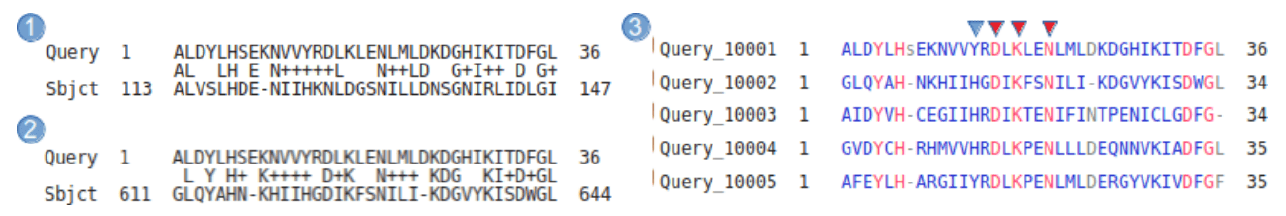
\includegraphics[width = \textwidth]{figs/msa.png}
\caption{\textbf{Pairwise vs MSA}. Se utilizó un fragmento del dominio quinasa de AKT7 humano (P31749) como consulta para buscar en una base de datos de proteínas archaca. (1) Alineación de AKTI y una ATPasa de la familia AAA (WP\_109940497.1) de \textit{Methanospirillum stamsii}. (2) Alineamiento del mismo fragmento de AKTI con una serina/treonina-proteína quinasa (OPY23844) de \textit{Methanobacterium sp}.. (3) MSA del sitio activo de 5 serina-treonina quinasas distantes. En flecha roja los residuos conservados en las 5 secuencias alineadas. Las puntas de flecha rojas marcan tres posiciones invariantes conservadas en todas las Ser/Thr-cinasas conocidas, el residuo Asp (D en esta tríada es el residuo del sitio activo. La punta de flecha azul marca una posición que está ocupada por His o Tyr en todas las proteínas conocidas de esta superfamilia).}
\label{fig:msa}
\end{figure}

\section{Métodos y esquemas de puntuación para la alineación de secuencias múltiples}
Como se explica en el capítulo anterior, la alineación óptima por pares puede lograrse eficazmente mediante algoritmos de programación dinámica. Estos métodos se basan en la construcción de una matriz $n \cdot m$, donde n y m corresponden a la longitud de las secuencias alineadas, y su complejidad en tiempo de ejecución es del orden de $O(n \cdot m)$ u $O(n^2)$ suponiendo que $n \sim m$. La extensión de este método a MSA es trivial. Por ejemplo, para tres secuencias de longitudes n, m y k, construiríamos una matriz $n \cdot m \cdot k$ que contenga las puntuaciones parciales óptimas para el alineamiento de tres posiciones. Sin embargo, la complejidad temporal en este caso sería de $O(n \cdot m \cdot k)$ u $O(n^3)$ suponiendo que $n \sim m \sim k$. De forma más general, para s secuencias de longitud n, la complejidad temporal sería $O(n^s)$ que crece exponencialmente con el número de secuencias. Por lo tanto, aunque este enfoque conduciría a un MSA óptimo, es poco práctico para más de unas pocas secuencias. Por este motivo, los métodos «simultáneos» no pueden aplicarse a problemas reales de MSA y se aproximan mediante métodos heurísticos que reducen el tiempo de cálculo pero no garantizan encontrar el alineamiento múltiple óptimo. Uno de los programas más populares para realizar MSA es ClustalW. Es un ejemplo de una familia de algoritmos que siguen una estrategia progresiva o jerárquica. Los métodos progresivos funcionan en tres pasos (véase la figura \ref{fig:clustalw}):
\begin{enumerate}
\item En el primer paso, este programa computa todos los posibles alineamientos por pares y calcula una puntuación bruta para cada alineamiento. La puntuación puede ser simplemente el porcentaje de identidades o medidas más sofisticadas.
\item A continuación, se realiza un análisis jerárquico de conglomerados en la tabla de puntuaciones por pares del paso anterior. Esta técnica produce un árbol guía o dendrograma que agrupa las secuencias según su similitud.
\item Por último, las secuencias se alinean progresivamente siguiendo la topología del árbol generado en el paso anterior. Así, se alinean las dos secuencias con la puntuación de similitud más alta y, a continuación, la secuencia siguiente se añade al alineamiento por pares o se utiliza en otro alineamiento por pares. Aunque no entraremos en detalles aquí, existen métodos rigurosos para alinear una secuencia contra un alineamiento. Imaginemos que la secuencia se alinea con una secuencia consenso derivada del alineamiento. El MSA puede representarse mediante estructuras matemáticas denominadas perfiles. En algún momento, los perfiles se alinean con los perfiles. Por último, el MSA se genera siguiendo el árbol guía desde los nodos más terminales hasta la raíz.
\end{enumerate}

\begin{figure}[htbp]
\centering
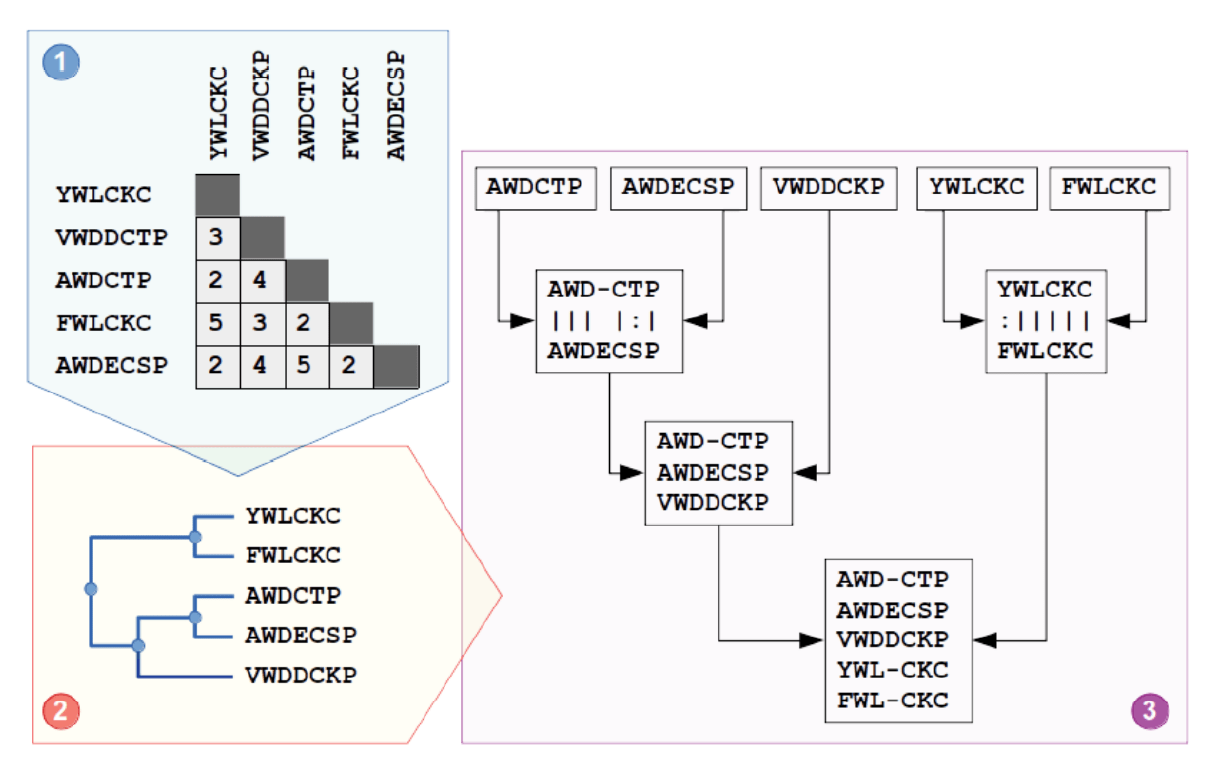
\includegraphics[width = \textwidth]{figs/clustalw.png}
\caption{\textbf{Métodos progresivos para el MSA}. Para producir un MSA de las secuencias YWLCKC (secuencia A), VWDDCTP (secuencia B). AWDCTP (secuencia C), FWLCKC (secuencia D) y AWDECSP (secuencia E), los métodos progresivos comparan primero todos los pares de secuencias (no mostrados) y registran la puntuación de cada alineamiento por pares (1). A continuación, basándose en estas puntuaciones, el algoritmo produce un árbol guía (2). Por último, las secuencias se alinean progresivamente empezando por las más cercanas. En cada paso del proceso, el algoritmo sigue la topología del árbol desde las hojas hasta la raíz, añadiendo nuevas secuencias o alineaciones en cada nodo del árbol (3).}
\label{fig:clustalw}
\end{figure}

Además de ClustalW, otras herramientas implementan variaciones de este algoritmo progresivo. Por ejemplo, ClustalW utiliza programación dinámica para el alineamiento por pares inicial, que es preciso pero puede ser lento para un gran número de secuencias. Por esta razón, otros métodos, como Kalign, cuentan el número de k-mers compartidos por las secuencias para calcular la distancia entre todos los pares. La ventaja de este método es que no es necesario alinear las secuencias para generar la matriz de distancias.

Uno de los problemas de los métodos progresivos es que el orden en que se añaden gradualmente las secuencias puede tener un fuerte impacto en el MSA final. Además, cuando se produce un error en un alineamiento intermedio, suele propagarse en los alineamientos posteriores. Esto es especialmente cierto en el caso de los gaps. Para mitigar estos problemas, diferentes algoritmos han adoptado variaciones en el procedimiento general, pero no las discutiremos aquí. Otro problema no resuelto en MSA es cómo calcular la puntuación. Se han propuesto varias estrategias:
\begin{itemize}
\item Scoring basado en una secuencia de referencia: $S_{MSA} = S_{AB} + S_{AC} + S_{AD} + S_{AE} $
\item Scoring basado en el dendograma: $S_{MSA} = S_{AB} + S_{CD} + S_{CD/E} + S_{AB/CDE}$
\item Scoring basado en la suma de alineamientos por pares: $S_{MSA} = S_{AB} + S_{AC} + S_{AD} + S_{AE} + S_{BC} + S_{BD} + S_{BE} + S_{CD} + S_{CE} + S_{DE}$
\end{itemize}

En resumen, aún no se ha resuelto el problema de calcular un MSA óptimo en un tiempo práctico. Mientras tanto, se han desarrollado varios enfoques heurísticos para calcular soluciones aproximadas que no garantizan ser la mejor solución posible.

Hasta ahora nos hemos centrado en el MSA de proteínas, sin embargo, el alineamiento múltiple de secuencias de regiones genómicas merece especial atención debido a la creciente cantidad de genomas completos disponibles y a su relevancia para identificar regiones genómicas reguladoras y comprender la variabilidad genética interindividual e interespecífica. Aunque no entraremos en detalles, la alineación de regiones genómicas plantea retos específicos. Por ejemplo, los genomas contienen un gran número de regiones repetitivas que son difíciles de alinear con precisión. Además, aunque la secuencia de determinadas regiones del genoma pueda conservarse en diferentes especies, a menudo la posición relativa de las distintas porciones del genoma no se conserva debido a reordenamientos genómicos. Por último, los MSA proteínicos suelen estar formados por un gran número de secuencias relativamente cortas, mientras que ocurre lo contrario con los MSA genómicos. Por todas estas razones, la alineación genómica requiere métodos de MSA especializados. Uno de ellos es MLAGAN, que se basa en un método progresivo similar al utilizado por ClustalW, y MULTIZ, utilizado para producir el MSA genómico que muestra el navegador del genoma de la UCSC.

\subsection{Ejemplo: FOXP2}
FOXP2 es un factor de transcripción. Al realizar un alineamiento de múltiples secuencias, se observan algunos residuos que presentan unos cambios únicos en humanos y son los que nos aportan la capacidad de comunicación como el habla. Además, individuos que tienen mutados esos individuos presentan un desorden del lenguaje. Por tanto, esos residuos son clave, y esto se demostró en ratones a los que se les cambió esos residuos concretos. Visto que esos cambios aparecen específicamente en humanos y que introducidos en ratones producen un comportamiento similar al habla, se analizó la filogenia y se observó exclusivamente en \textit{Homo sapiens} y Neandertales, pero no en otros primates.

\begin{figure}[htbp]
\centering
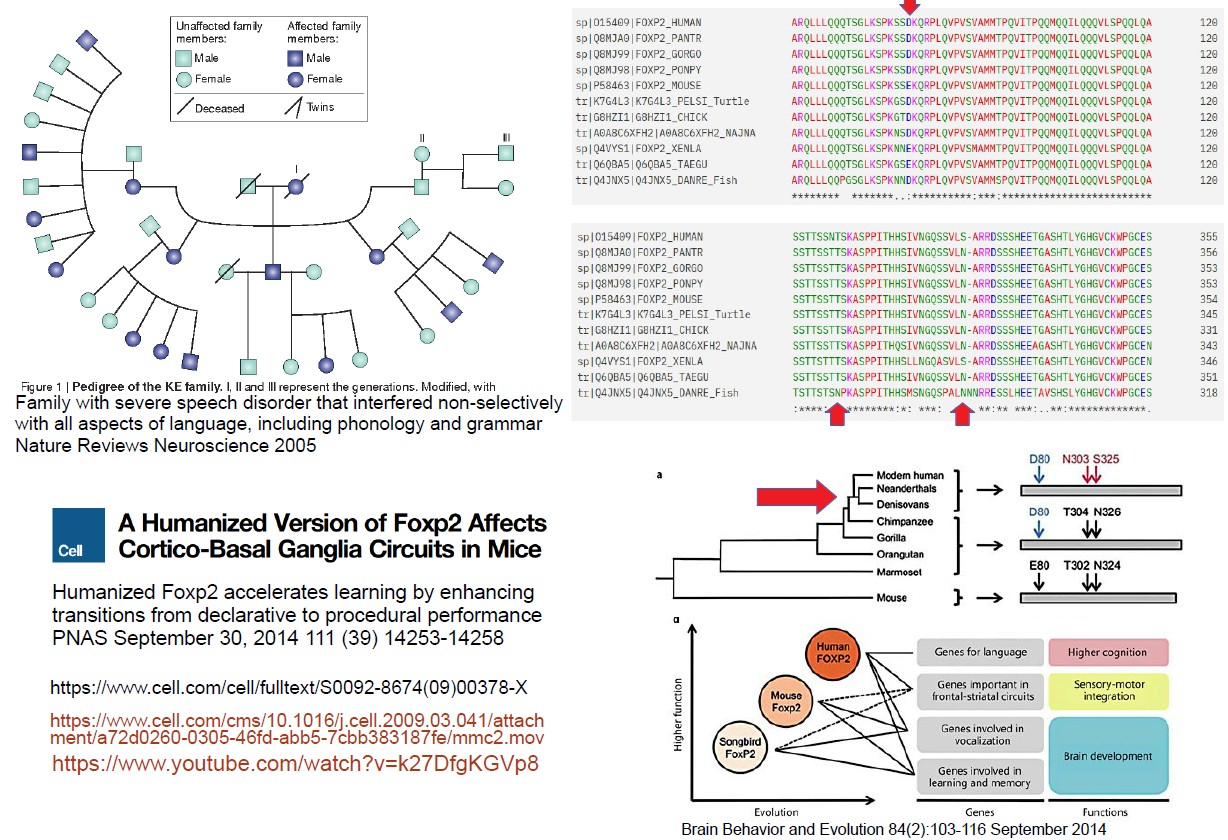
\includegraphics[width = \textwidth]{figs/foxp2.png}
\caption{Ejemplo del factor de transcripción FOXP2}
\end{figure}

\section{Representación de MSA}
Como se ha explicado anteriormente, el MSA puede utilizarse para identificar motivos/dominios funcionales y/o estructurales en un grupo de secuencias. Y lo que es más importante, una vez que hemos identificado ese motivo/dominio, puede utilizarse para buscar en bases de datos e identificar otras proteínas que compartan ese (nuevo) motivo y, como veremos, esas búsquedas son mucho más sensibles que las basadas en una secuencia de consulta. Sin embargo, para realizar dichas búsquedas, necesitamos una forma de representar el motivo/dominio revelado en el MSA. Existen varias formas de representar una región conservada, como se explica a continuación.
